%!TEX root = ../thesis.tex
%*******************************************************************************
%****************************** Third Chapter **********************************
%*******************************************************************************
\chapter{Neural tensor factorisation}

% **************************** Define Graphics Path **************************

\ifpdf
     \graphicspath{{Figs/Chapter3/}}
\else
    \graphicspath{{Chapter3/Figs/Vector/}{Chapter3/Figs/}}
\fi

Knowledge graphs (KGs) are a framework used to represent logical structure in data \unskip ~\citep{koller2007introduction}. The resource description framework (RDF) formalism, subject-predicate-object, is especially useful in encoding the relational data representation by KGs, dyadic relationships between entities expressed nodes and edges.\ Recently approaches to combine statistical learning focused on feature representation of data, with relational data representation have been attempted in a KG link prediction setting \unskip~\citep{kazemi2018simple, chang2014typed, kang2012gigatensor}, statistical relational learning (SRL). Tensor factorisation has been explored as an approach to link prediction \unskip ~\citep{nickel2011three, bordes2013translating, trouillon2016complex}.\ This approach has shown promise as a machine learning approach in domains that are high-dimensional and sparse. It is also compute efficient, and lends itself to GPU computation common in modern machine learning workloads. \par

\noindent KG tensor factorisation decomposes relational score tensors into an entity matrix, a relational tensor and transposed entity matrix.\ The entity matrix is composed of entity vectors, latent entity representations consisting of trainable parameters that need to be learned. The relational tensor is composed of relational matrix slices, latent relational representations also consisting of trainable parameters that need to be learned, corresponding to the set of relation types in the KG. The product between the entity matrix, the relational tensor and the transposed entity matrix is the bilinear tensor product. In practise this is performed by expressing KG facts (entity-relation-entity) as RDF triples (subject-predicate-object). Then generating a subject-predicate vector and taking the inner product of this vector with all object vectors, illustrated in Figure 3.1. This operation generates a relational score tensor with unnormalised scores of potential relationships between entities, indexed by relation.\ A probability of relation in the interval $ (0, 1] $ is then computed for each score using a sigmoid function. During inference, probabilities are sorted in descending order to rank the potential for possible relationships. \par

\begin{figure}[H]
   	\centering
    	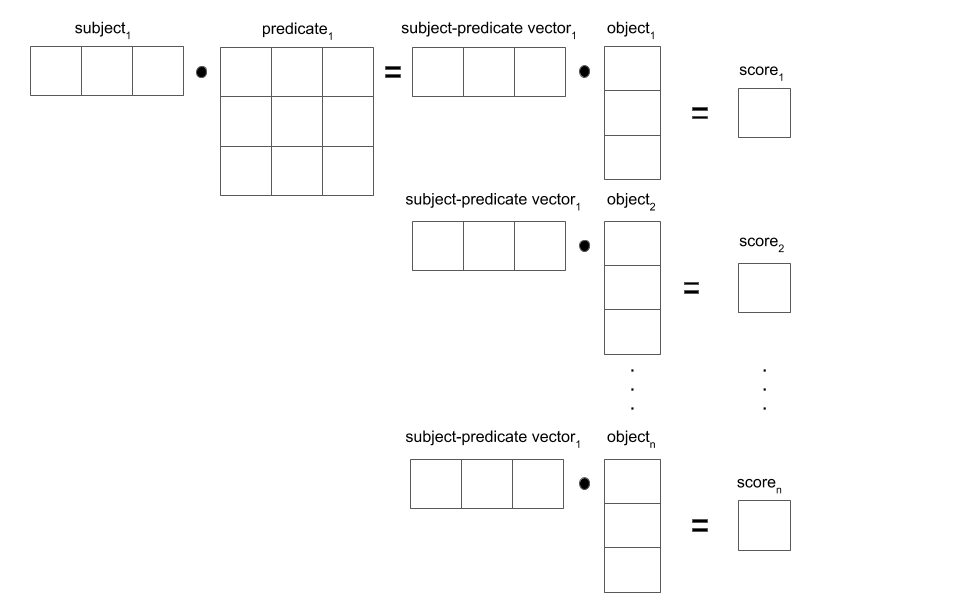
\includegraphics[width=0.7\textwidth, height=0.4\textwidth]{inference}
	\captionsetup{justification=centering}
	\caption{Relation prediction between two entities. $ subject_1 $ and $ object_1 $ are two distinct entities, and $ predicate_1 $ is a relation from the set of relations in the KG. A product is taken between $ subject-predicate \; vector_1 $ and all $ objects $ in the KG.}
\end{figure}

\noindent Previous tensor factorisation approaches focused on limiting the total number of model parameters in order to scale to large KGs. This approach was often at the expense of complex entity-relational interaction modelling.\ The neural tensor network (NTN) \unskip~\citep{socher2013reasoning}, a nonlinear extension of tensor factorisation, was the first successful attempt to take advantage of the expressiveness of neural compositional models. It relies on using a recursive network (RCN) \unskip ~\citep{pollack1990recursive} to output a compositional score between two entities, adding that score to the bilinear tensor product, and passing the result through a nonlinearity to compute a relational score. A hyperbolic tangent function is then applied to generate a measure of confidence in a potential relationship between the two entities.\par

\noindent Convolutional entity-relational modelling (ConvE) \unskip~\citep{dettmers2018convolutional} was similarly effective at extending tensor factorisation.\ ConvE lengthwise concatenates a subject vector and predicate vector into an subject-predicate matrix, then applies a 2-dimensional ($ 2D $) convolution operation on this matrix, convolutional tensor factorisation. A product is then taken between the generated subject-predicate vector and an object vector, to compute a relational score.\ Here a sigmoid function is applied to generate a probability of a potential relationship between the two entities. \par 

\noindent An alternative approach to convolutional tensor factorisation is HypER \unskip~\citep{balazevic2019hypernetwork}. It models entity-relational interactions by using a hypernetwork \unskip~\citep{ha2016hypernetworks} to generate $ 2D $ relation-specific convolutional filters (predicate matrices). A $ 2D $ convolution is then taken between a subject vector and predicate matrix. Finally an inner product is taken between the generated subject-predicate vector and an object vector, which computes a relational score. Once again a sigmoid function is then applied to generate a probability of a potential relationship. \par

\noindent In the rest of this chapter we assess the NTN model and attempt a simple improvement by applying adaptive moment estimation (Adam) optimisation \unskip ~\citep{kingma2014adam}, early stopping \unskip ~\citep{prechelt1998early} and hyperparameter random search \unskip ~\citep{bergstra2012random} to the training algorithm. We then propose HypER+, an extension of the HypER model which compensates for covariate shift introduced by the hypernetwork when generating relation-specific convolutional filters. Finally we extend HypER+ by intialising entity and relation model embeddings using pre-trained word vectors from the GloVe language model \unskip ~\citep{pennington2014glove}. In doing so we take advantage of semantic information contained in these vectors. 


% **************************** First Section **************************

\section{Neural tensor networks}

\subsection{Nonlinear latent feature modelling}
Nickel et al. \unskip ~\citep{nickel2011three} introduced the bilinear tensor product for relational scoring, in a model called RESCAL. This model makes use of entity vectors and a relational tensor, where each relation type is modelled as a matrix slice of the tensor. RESCAL is defined as follows:
\begin{equation}
	f_{i, k, j} = e_i^TW_ke_j = \sum_{a=1}^{H_e}\sum_{b=1}^{H_e}W_{a,b,k}e_{ia}e_{jb}
\end{equation}

\noindent where $ f_{i,k,j} $ is the relational score, $ e_i $ is the subject vector and $ e_j $ is the object vector, entity representations implemented as model embeddings. $ W_k $ is the predicate matrix for relation $ k $, a relation representation implemented as a model embedding. Entity-relational interactions are modelled using the vector-matrix product between the subject vector and predicate matrix, generating a subject-predicate vector. A relational score is then computed by taking the inner product between the subject-predicate vector and the object vector. RESCAL is thus a linear tensor factorisation composition. \par

\noindent A natural extension to this model is to include a nonlinearity for relational scoring. This extension was introduced by Jenatton et al. \unskip ~\citep{jenatton2012latent}. Their model uses a sigmoid nonlinearity to generate a probability of a possible relationship from the relational score computed using the bilinear tensor product. The model is defined as follows:
\begin{subequations}
	\begin{gather}
		n_{i,j,k} = e_i^TW_ke_j \\
		\mathbb{P}\left [ R_j(S_i, O_k) = 1 \right ] = \sigma(n_{i,j,k})
	\end{gather}
\end{subequations}

\noindent where $ n_{i,j,k} $ is the relational score, $ \sigma(t) = 1/(1 + e^{-t}) $ is the sigmoid function, a value in the range $\in \left ( 0, 1 \right ]$, and $\mathbb{P}$ is the probability of a potential relationship between subject $ S_i $ and object $ O_k $, indexed by relation $ R_j $. This model introduces nonlinear relational scoring to latent feature modelling based link prediction. 


%********************************************* Recursive neural tensor factorisation **************************************************

\subsection{Recursive neural tensor factorisation}

Chen et al.  \unskip ~\citep{socher2013reasoning} introduce nonlinear tensor factorisation by adding recursive entity representations in the composition of the relational score. Recursive networks (RCNs) try to capture the rules for word combinations by constructing a composition tree between words, in a sequence of words \unskip ~\citep{socher2012semantic}, illustrated in figure 3.2. \par

\begin{figure}[H]
   	\centering
    	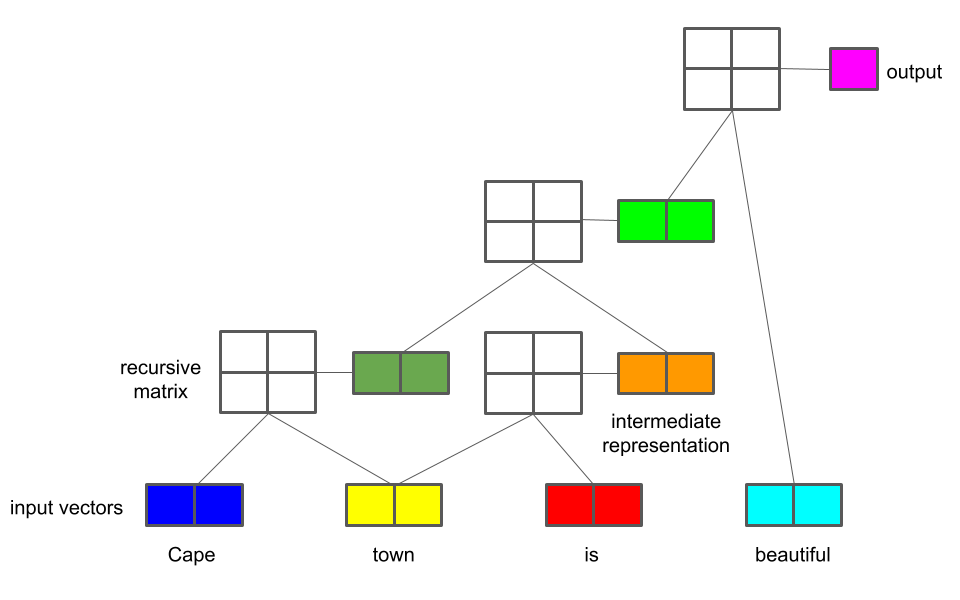
\includegraphics[width=0.6\textwidth, height=0.3\textwidth]{recursive_network.png}
	\captionsetup{justification=centering}
	\caption{Recursive network which constructs a composition tree between inputs. It begins with a full tree and is pruned during training to obtain the optimal structure.}
\end{figure}

\noindent The NTN model tries to take advantage of these compositional rules by adding them to the bilinear tensor product, illustrated in Figure 3.3, and is defined as follows:
\begin{equation}
	g_{i,k,j} =  u_k^Tf(e_i^TW_k^{\left [1:m \right ]} e_j + V_k \left [ \begin{matrix} e_i \\ e_j \end{matrix} \right ] + b_k)
\end{equation}

\noindent where $ g_{i,k,j} $ is the relational score tensor, $ u_k^T \in \mathbb{R}^{1 \times m} $ is an output layer of trainable prameters, and $ f $ is the hyperbolic tangent function. $ e_i^TW_k^{\left [1:m \right ]} e_j $ is the bilinear tensor product between subject vector $ e_i^T \in \mathbb{R}^{1 \times n} $ and object vector $ e_j \in \mathbb{R}^{n \times 1} $, computed for relations $ W_k \in \mathbb{R}^{n \times n} $, where $ k \in \{1 \dots \; m \} $, and $ b_k $ is the bias. $ \; V_k \left [ \begin{matrix} e_i \\ e_j \end{matrix} \right ] $ is the recursive entity composition, where $ V_k \in \mathbb{R}^{k \times 2n} $ is a matrix of trainable parameters, and the matrix-vector product is taken between $ V_k $ and the concatenation of the subject and object vectors. A row of matrix $ V_k $ corresponds to relation $ k $. The output of a subject $ i $ and object $ j $ input, $ \{ e_i, \; e_j \} $, is a vector of relational scores $ \{ s_{i,1,j}, \; \dots, \; s_{i,m,j} \} $ for all predicates $ W_k $ of the KG. 

\begin{figure}[H]
   	\centering
    	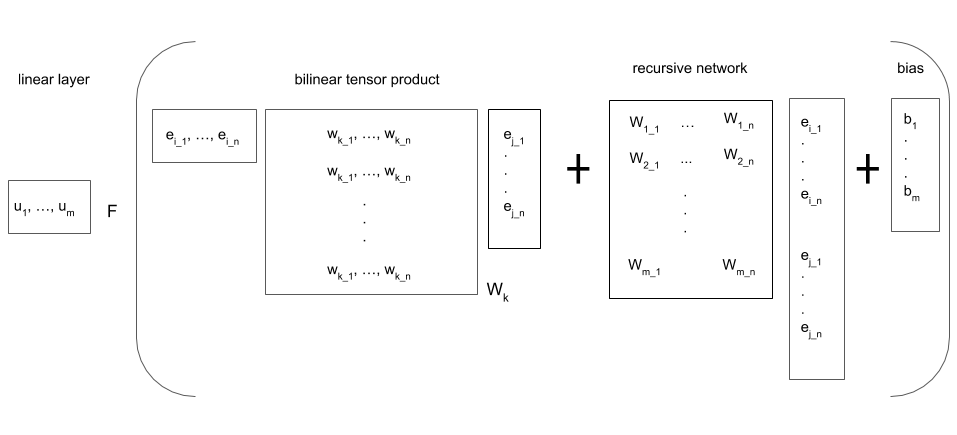
\includegraphics[width=0.7\textwidth, height=0.4\textwidth]{recursive_neural_tensor_network.png}
	\captionsetup{justification=centering}
	\caption{Recursive neural tensor network. This model computes the bilinear tensor product, and adds it to a recursive composition of entities and a bias to compute a relational score between the entities. The final result is squashed using a hyperbolic tangent function.}
\end{figure}

\noindent The contrastive max-margin loss is minimised during training. This loss computes a confidence magnitude on a correct sample (a fact present in the KG), and a confidence magnitude on a corrupt sample (a randomly generated fact not present in the KG). The correct and corrupt samples are used by the loss function as follows:
\begin{equation}
	J(\si{\ohm}) =  \sum_{i=1}^N \sum_{c=1}^C \max(0,1 - g(T^{(i)}) + g(T_c^{(i)})) + \lambda \left \lVert \si{\ohm} \right \rVert_2^2
\end{equation}

\noindent where $J$ is the loss value, $\si{\ohm}$ contains the trainable parameters $u, W, V, b $, and $ E $. $N$ is the number of training sample triplets, and $ C $ is the number of randomly corrupted facts. $ g(T^{(i)}) $ is the confidence in the true fact computed by the model, and $ g(T_c^{(i)}) $ is the confidence in the corrupt fact computed by the model. Finally $\lambda\left\lVert \si{\ohm} \right\rVert_2^2$ is the ridge ($L_2$) regression regulariser. \par

\noindent The NTN model training algorithm also makes use of pre-trained word vectors, from a language model by Turian et al. \unskip ~\citep{turian2010word}, to initialise entity embeddings. These are 100-dimensional vectors, which are aggregated from the set of words that represent an entity. For example for the entity \textit{homo sapiens}, the resulting entity embedding is $V_{homo \; sapiens} = 0.5(V_{homo} + V_{sapiens})$. These entity embeddings are trainable, and updated using backpropagation to generate a distributed representation of words that aligns with the KG of the particular application. \par

\subsection{Training algorithm optimisation} 

Overfitting can be a concern for models with large numbers of parameters. This problem results in poor generalisation to testing data by the model. It can occur when training has progressed beyond the optimal point, and the model parameters begin to bias toward the training data. High model bias is revealed by good model performance on training data, and poor performance on validation data. Early stopping \unskip~\citep{prechelt1998early} is often used to prevent this and encourage generalisation. \par

\noindent Neural model training can suffer from slow convergence when using stochastic gradient descent, mini-batch optimisation, and regularisation techniques such as dropout. Neural models can also suffer from insufficient signal to update parameters, a problem known as sparse gradients. Adaptive moment estimation (Adam) is a first order gradient-based stochastic optimisation algorithm that compensates for these problems \unskip ~\citep{kingma2014adam}. It computes the adaptive learning rates for parameters using the first and second order moments of the gradient, combining the advantages of AdaGrad ~\citep{duchi2011adaptive} and RMSprop ~\citep{tieleman2012lecture}. Adam efficiently regulates the size of parameter updates, accelerating toward local optima, and remaining small in sparse regions and where the gradient signal is small. \par

\noindent Setting model hyperparameters remains a challenge in neural model training. A simple method proposed to address this problem is hyperparameter random search \unskip ~\citep{bergstra2012random}, the process of defining intervals for model hyperparameters, and randomly sampling from those intervals for a finite number of training runs (experiments). This approach improves on grid search, a brute force process that iterates through combinations of hyperparameter intervals, as models often match or exceed performance in a fraction of the training time. It takes advantage of the fact that for most datasets, only a subset of the hyperparameters contribute meaningful variance in model performance, eliminating the need for an exhaustive search over a large combinatorial space. \par

\subsection{Training algorithm}

Doss et al. \unskip~\citep{Doss2015} reimplemented the NTN model in TensorFlow \unskip ~\citep{abadi2016tensorflow}. This model underperforms compared to the original model, relying on AdaGrad optimisation and the same hyperparameters. We apply early stopping, Adam optimisation as well as hyperparameter random search, in an attempt to improve performance. The new training algorithm is as follows: 

\medskip

\begin{algorithm}[H]
	Repeat for $ Z $ experiments using random uniform hyperparameter configuration \\
	\For{Epoch}{ 
		\SetAlgoLined
		\textbf{Input} 
		Training set \begin{math} D = \{(x_i, \; y_i)\}_{i=1}^N \end{math}, of samples and labels\;
  		\begin{math} S \gets sample(D, \; b) \end{math} // sample a mini-batch of size $ b $ from training set $ D $\\
		\For{S}{
	 		\For{(x, y) $ \in S $}{
     				$ y^{'}_{correct} \gets predict(x) $ \\ // for $ \{ e_i, e_{jt} \} $ predict relational score $ g(T^{(i)}) $ for sample \\
				$ y^{'}_{corrupt} \gets predict(x) $ \\ // for $ \{ e_i, e_{jc} \} $ predict relational score $ g(T_c^{(i)}) $ for sample \\
				$ e \gets contrast(y^{'}_{correct}, \;  y^{'}_{corrupt}) $ // compute error
     			}
			Update model w.r.t. \begin{math}  e \end{math} // using Adam optimser \\
			\For{Validation}{
				Check validation score at previous iteration, $ vScore_{t - 1} $ \\
				If  $ vScore_{t} < vScore_{t - 1} $ \\
					Stop training. // early stopping
			}
		}
	}
	\caption{Optimised NTN training algorithm}
\end{algorithm} 


% **************************** Second Section **************************

\section{Hypernetwork tensor factorisation}

\subsection{Convolutional factorisation}

ConvE introduced the convolutional operator to neural tensor factorisation \unskip ~\citep{dettmers2018convolutional}. Specifically, this operator increases expressiveness in entity-relation interaction modelling by using 2-dimensional convolutions, which are particularly effective at modelling the interactions of entities involved in a large number of relations. ConvE concatenates subject and predicate matrices along the row axis, creating a 2-dimensional entity-relational matrix. Convolutional filters are then applied to this representation, producing feature maps which are flattened by a fully connected layer. The dot product of this generated representation is then taken with the object vector, computing an unnormalised relational score between the subject and object, before a sigmoid function is applied to produce a probability of relational plausibility. The model is defined as follows:
\begin{equation}
	\psi_r(e_s, \; e_o) = g(vec(f(\left [ \overline{e_s}; \; \overline{r_r} \right ]*w))W)e_o
\end{equation}

\noindent where $ \psi_r $ is the relational score, $ e_s $ is the subject, $ e_o $ is the object, and $ r $ is the predicate. $ f $ is the concatenation operation between the subject and predicate, $ w $ contains the 2-dimensional convolutional filters, and $ * $ is the convolutional operator. $ vec $ reshapes the feature map tensor into a vector which is passed through a fully connected layer parameterised by $ W $, and then $ g $, a ReLU nonlinearity. ConvE is thus a convolutional tensor factorisation. 

\begin{figure}[H]
   	\centering
    	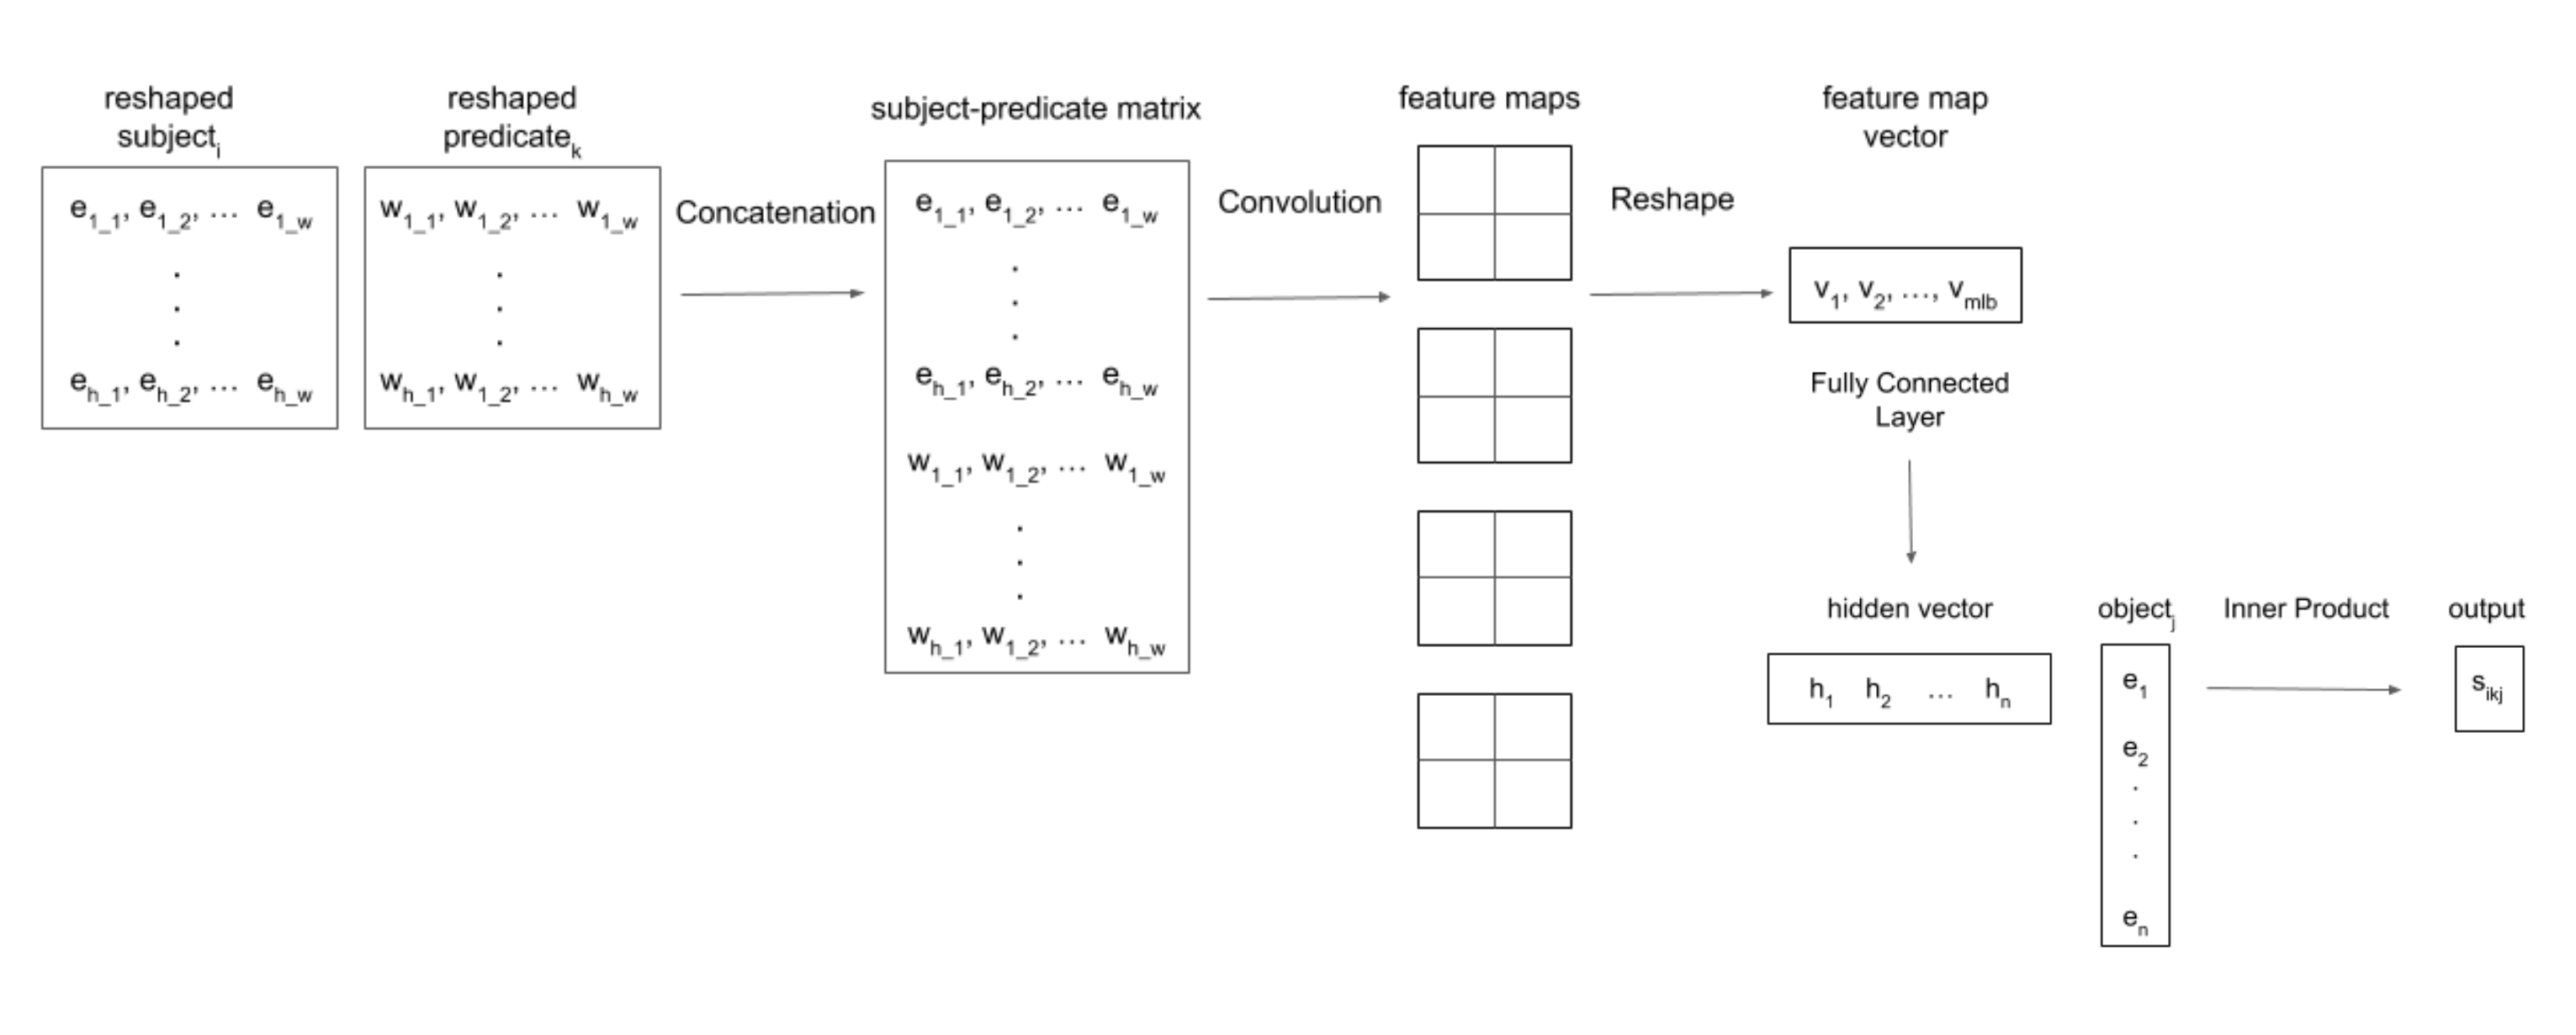
\includegraphics[width=0.7\textwidth, height=0.4\textwidth]{convolutional_entity_representations_final}
	\caption{Convolutional entity representations.}
\end{figure}

\newpage

\noindent The computed relational probability is defined as follows: 
\begin{equation}
	\mathbb{P} = \sigma(\psi_r(e_s, \; e_o)) 
\end{equation}

\noindent The binary cross-entropy objective is minimised during training. This objective is particularly effective as we expect only a single true class (a single object from the set of all entities) during inference, modelled as $1$, and every other class to be false, $0$. The objective is defined as follows:
\begin{equation}
	L(p, \; t) =  -\frac{1}{N}\sum_i(t_i \cdot log(p_i) + (1 - t_i) \cdot log(1 - p_i))
\end{equation}

\noindent where $ L $ is the loss value, $ p_i $ is the relational probability computed by the model, and $ t_i $ is the target. $ N $ is the batch size, and $ i $ is the sample index.

\subsection{Hypernetwork factorisation}

Hypernetworks are meta networks that generate parameters for a main network \unskip ~\citep{ha2016hypernetworks}. The networks essentially index the parameters of a main network as a configuration given input. This input is typically in the form of an embedding vector that describes all the weights of a given layer. The configuration is learned given a scenario experienced by the main network, for example when performing sequence prediction it may be advantageous for the main network to change its behaviour (parameter configuration) depending on the sequence window. The hypernetwork model can be defined as follows: 
\begin{equation}
	K_j = g(z_j), \quad \forall j = 1, \dots, D
\end{equation}

\noindent where $ K_j $ contains the parameters of layer $ j $, $ g $ is the hypernetwork composition, and $ z_j $ is the hypernetwork input. \par

\noindent HypER is inspired by ConvE, and implements a convolutional operator that models entity-relational interactions \unskip ~\citep{balazevic2019hypernetwork}. It makes use of a hypernetwork to generate relation-specific convolutional filters. The subject and relational filter are then used in a convolution operation to generate latent representations which are flattened by a fully connected layer. The dot product of this generated representation is then taken with the object vector, producing a measure of confidence in the relation, before a logistic sigmoid is applied to compute a probability of plausibility. The model is defined as follows: \newpage

\begin{equation}
	\phi_r(e_s, \; e_o) = f(vec(e_s * (vec^{-1}(w_rH)))W)e_o
\end{equation}

\noindent where $ \phi_r $ is the relational score, $ e_s $ is the subject, and $ e_o $ is the object. $ w_r $ is the predicate input and $ H $ is the parameterised matrix of the fully connected layer of the hypernetwork, $ vec^{-1} $ is the transformation that reshapes the output of the hypernetwork into a set of relation-specific convolutional filters. $ * $ is the convolutional operator, $ vec $ reshapes the feature map tensor into a vector which is passed through a fully connected layer parameterised by $ W $, and then $ f $, a ReLU nonlinearity. HypER is thus a hypernetwork convolutional tensor factorisation. 

\begin{figure}[H]
   	\centering
    	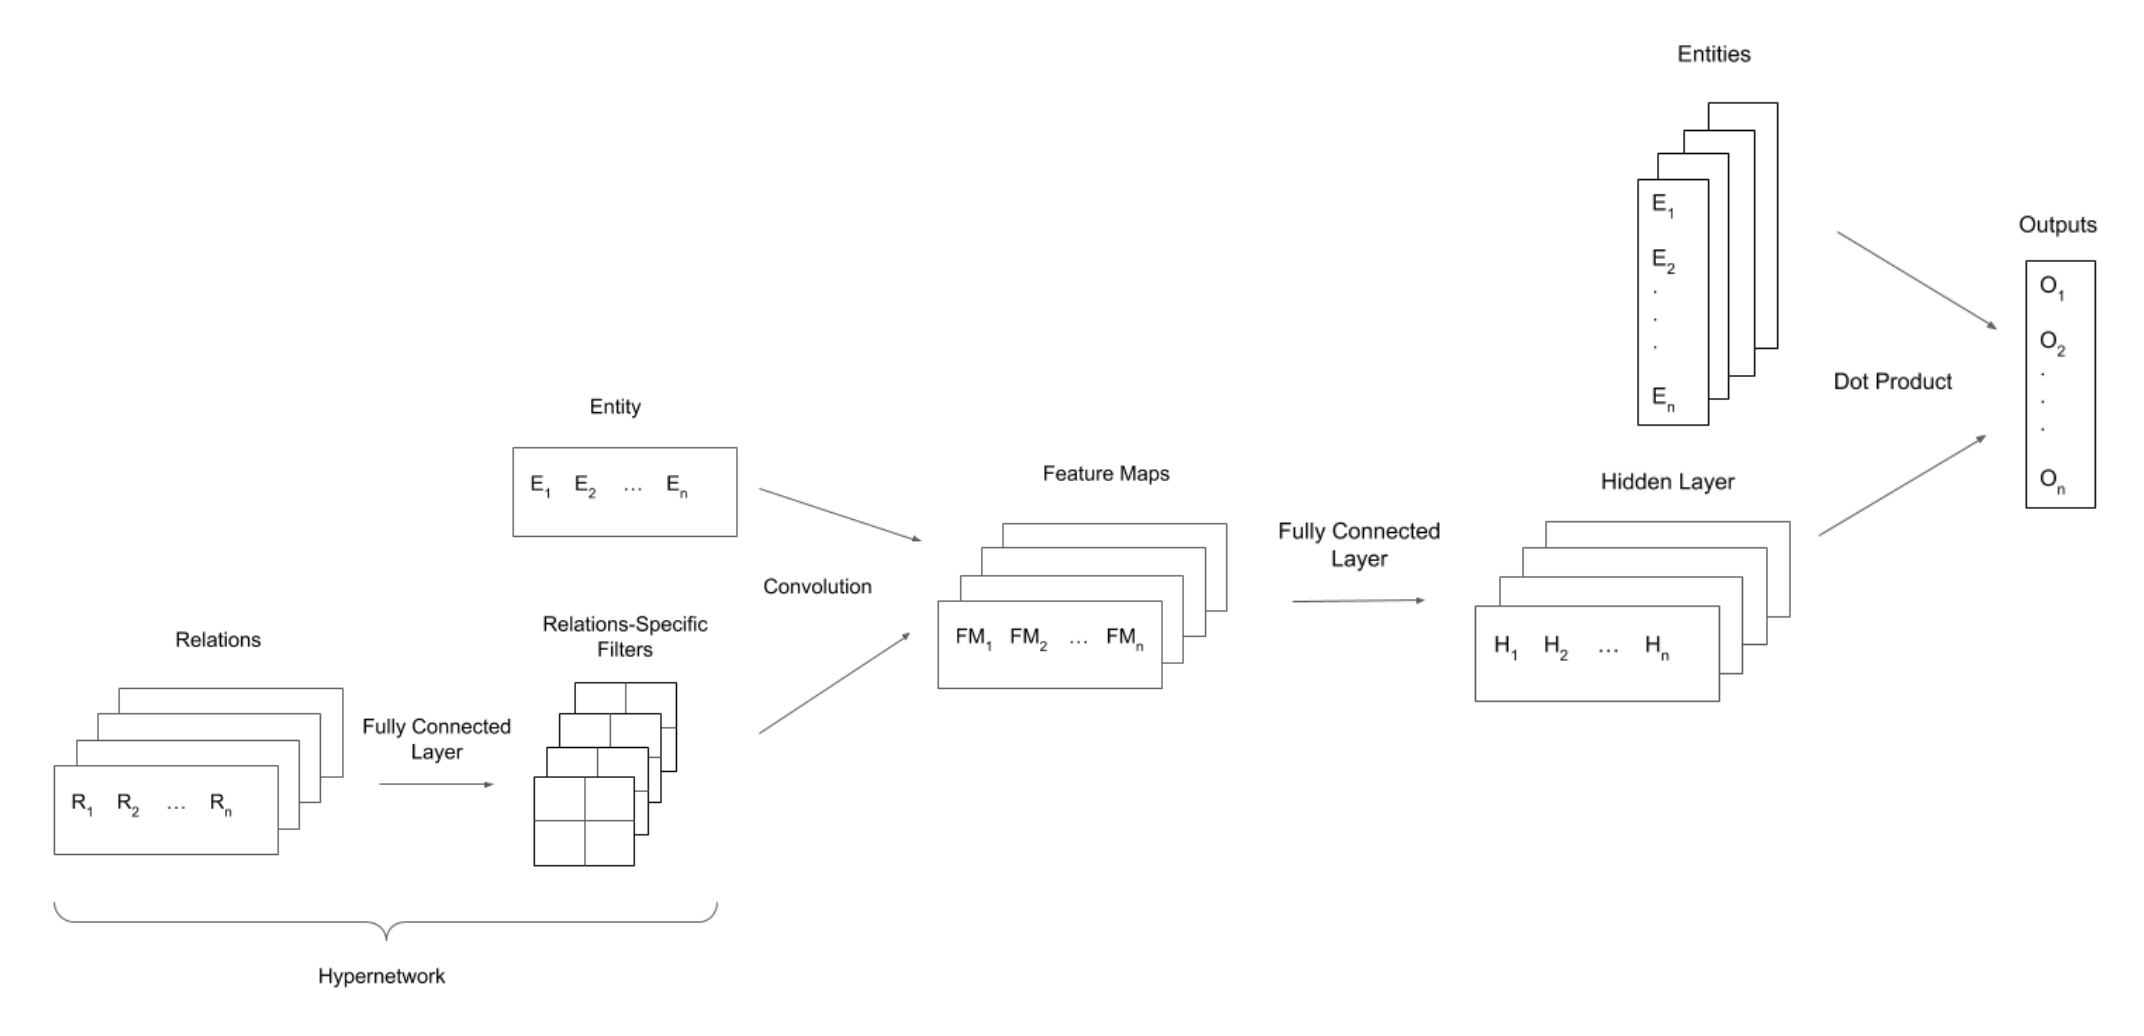
\includegraphics[width=0.7\textwidth, height=0.5\textwidth]{hyper_neural_tensor_network_final}
	\caption{Hypernetwork convolutional entity representations.}
\end{figure}

\noindent The computed relational probability is defined as follows: 
\begin{equation}
	\mathbb{P} = \sigma(\phi_r(e_s, \; e_o)) 
\end{equation}

\noindent The HypER training algorithm minimises the binary cross-entropy objective. Entities and relations are intialised using Xavier initialisation \unskip ~\citep{glorot2010understanding}, drawn from a uniform distribution with zero mean. \par

\noindent \textbf{HypER covariate shift}. We make the observation that hypernetworks may also suffer from covariate shift. Relational filters form inputs to the main convolutional network. During training, the latent parameters of the relations change, altering the input distribution of the generated relational filters. We consider whether this distribution shift makes it hard for the hpernetwork to learn parameters good at creating relational filters, given an input signal not representative of the underlying training dataset distribution. We further consider that given the relational filters are used early (upstream) in the main network, the effect of their suboptimal representations is amplified. \par

\noindent To address this problem, we introduce relational input batch normalisation. This operation performs normalisation on relational input mini-batches during training, such that each batch has zero mean and unit variance, regulating hypernetwork input. Population mean and variance are used to regulate input during inference. We adjust the HypER model accordingly, and call the adjusted model HypER+. \par

\bigskip

\begin{algorithm}[H]
	\SetAlgoLined
	\textbf{Input} 
	Training set \begin{math} D = \{(x_i, y_i)\}_{i=1}^N \end{math}, of input features and output labels\;
	Intialise parameters $w \in \mathbb{R}$, for model \begin{math} M(w) \end{math} // e.g. random normal initialisation \\
	\For{Epoch \begin{math} k = 1 \dots \; K  \end{math}}{
  		\begin{math} B \gets sample(D, s) \end{math} // sample minibatch of size \begin{math} s \end{math} \\
	 	\For{(x, y) \begin{math} \in B \end{math}}{
			\begin{math} y'_j = BN_{\gamma_j,\beta_j, \mu_{Bj}, s_{Bj}}(x_j) \end{math} // Transformation of inputs to layer $ j $ for batch $ B $ \\
     			\begin{math} y' \gets predict(x, \; y') \end{math} // predict label for sample \\
			\begin{math} e \gets y' - y \end{math} // compute loss
     			}
		\begin{math} w \gets w - \lambda * \hat{\nabla}_{w} J_{e} (w) \end{math} // partial derivative update of model with respect to cost $e$ \\
		\begin{math} \theta \gets \theta \; \cup \;  \{\gamma_j, \beta_j\}  \end{math} // Optimize batch normalisation parameters for layer $ j $
	}
	\begin{math} E[x] \gets E[\mu_B]  \end{math}, \begin{math} E[\sigma] \gets E[s_B]  \end{math} // Average $ \mu $ and $ s $ over mini-batches B 
	\caption{Training HypER+ with batch normalisation}
\end{algorithm} \bigbreak
 
\noindent \textbf{Pre-trained word vectors}. We then pre-trained GloVe word vectors \unskip ~\citep{pennington2014glove} to the HypER+ training algorithm. We use these word vectors to initialise  200-dimensional embeddings, which are aggregated from the set of words that represent an entity or relation, the same method of aggregation used for pre-trained word vectors used during NTN training. Similarly, these word vectors are trainable, and updated using backpropagation.  

%********************************** %Third Section  **************************************

\section{Summary}

Neural tensor networks constitute an early successful attempt at using the expressive power of neural networks for link prediction. This model also makes use of RCNs, which try to model semantic compositionality, and makes use of pre-trained word vectors to improve link prediction performance. We apply modern stochastic and hyperparameter optimisation techniques to the NTN training algorithm, namely Adam and hyperparameter random search. \newline
Hypernetworks can be used to generate parameters for other networks. This approach has the effect of applying a configuration to a neural network, and changing its behaviour given indexing input. Hypernetworks were used to generate parameters for a convolutional network in the model HypER. Concretely, HypER generates relation-specific convolutional filters which are used in a neural factorisation approach to link prediction. We adjust HypER to compensate for the covariate shift caused by the hypernetwork and introduce HypER+. We then extend HypER+ to make use of GloVe pre-trained word vectors by initialising entities and relations using these embeddings. \newline
